	\subsection{Taxonomy of mobile virtualization techniques by \textit{Shuja}}
	
	\begin{figure}[H]
		\centering
		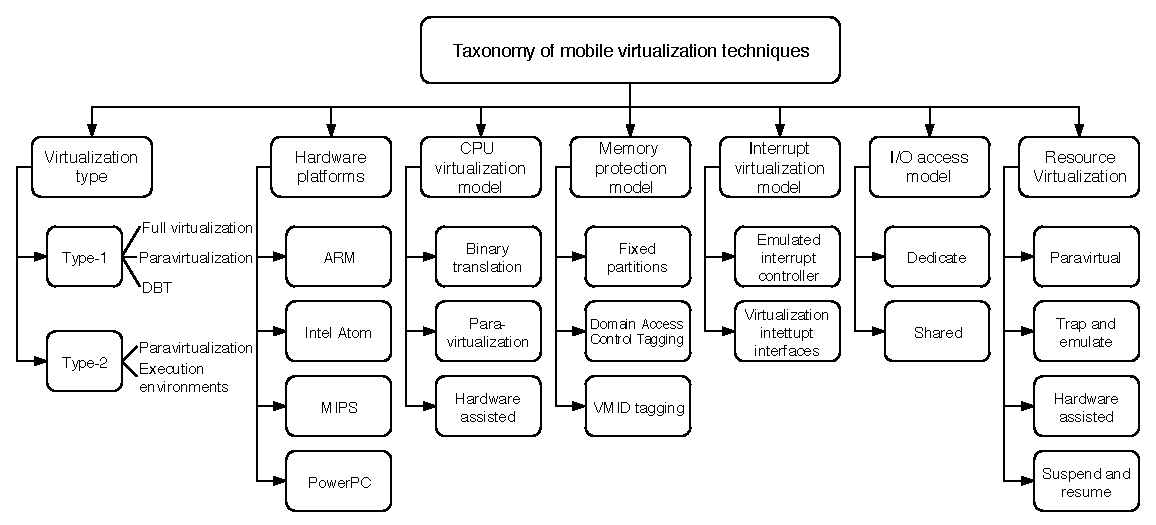
\includegraphics[width=8.5cm]{images/Shuja2016.pdf}
		\vspace{-0.2cm}
		\caption{Taxonomy of mobile virtualization techniques by \textit{Junaid Shuja, Kashif Bilal, Abdullah Gani and Samee Ullah Khan} in 2016 \cite{Shuja2016}.}
		\label{fig:TaxonomyByShuja}
	\end{figure}

	The study by Shuja et al \cite{Shuja2016} focuses on a taxonomy of mobile virtualization techniques with seven main categories: \textit{Virtualization type}, \textit{Hardware platforms}, \textit{CPU virtualization model}, \textit{Memory protection model}, \textit{Interrupt virtualization model}, \textit{I/O access model} and finally \textit{Network virtualization model}. 
	
	\textbf{Virtualization type} indicates the existence of two subcategories. As we have seen before, Type-1 is characterized by placing the guest OS directly on the underlying hardware and Type-2 by placing the guest OS on a underlying OS. \cite{Shuja2016, Zonghua2012}.
	
	\textbf{Hardware platform} presents the most popular manufacturers of infrastructure for mobile devices with are \textit{ARM}, \textit{Intel Atom}, \textit{MIPS}, and \textit{PowerPC}.
	
	\textbf{CPU virtualization model} shows different virtualization techniques such as \textit{Binary translation}, \textit{Paravirtualization} and \textit{Hardware assisted} virtualization used to trap and manage confidential instructions without privileges in ARM ISA. 
	
	\textbf{Memory protection model} shows three techniques such as Fixed partitions, Domain access control tagging, and VMID tagging. All of them focused on mobile devices with ARM ISA.

	\textbf{Interrupt virtualization model} shows that this process can be carried out using two techniques, either through "Emulated interrupt controller" or "Virtualization interrupt interfaces".

	\textbf{I/O access model} shows that it can be dedicated to a specific guest OS according to its priority or on the contrary, shared among all guest OSs. 

	\textbf{Network virtualization model} shows that it is possible to use four techniques such as: 1) \textit{Paravirtual} interfaces based on hypercalls, 2) \textit{Trap and emulate} procedure for network interface access, 3) \textit{Hardware assisted} multiple interface access to the guest OSs, and 4) \textit{Suspend and resume} routine. 
	
	Although Shuja et al.'s study \cite{Shuja2016} has considerable breadth in terms of the seven main categories discussed, they focus primarly on virtualization techniques for mobile devices, which limits the study's consideration of other important elements of the computing infrastructure.
	
	
	
	
	
	
	
	
	
	
	
	
	
	